% <-- chapter -->
\chapter{Configurazione del \textit{Server} \ok}
\label{ch:server}

\section{Overview della configurazione e prerequisiti \ok}
\label{sec:overview_server}

In questo capitolo andremo a installare e configurare \textit{OpenVPN server} sulla VPS di OVHCloud.

Per facilitare la configurazione e il testing, supponiamo di partire da una topologia che contiene solo il server OpenVPN e un generico client. Come da specifiche, il Server deve avere a disposizione un'IP pubblico (sezione \ref{subsec:vps-ovhcloud}); e il client deve essere il più generico possibile, lo supponiamo quindi sotto a un NAT (sezione \ref{subsec:macchina-cliente}).

Sappiamo inoltre che l'IP pubblico del Server è \code{51.178.141.119}, si avrà quindi una configurazione iniziale come in figura \ref{fig:diag-simple_ips}.


\newsavebox{\myimage}
\begin{figure}[H]
    \centering%
    \begin{subfigure}{0.49\textwidth}
        \centering
        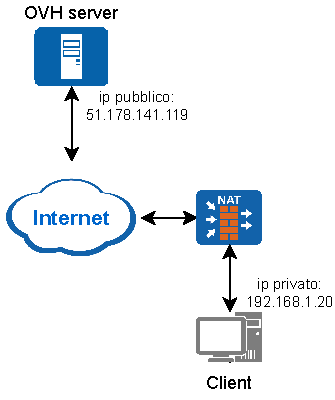
\includegraphics[width=0.8\textwidth]{immagini/diag-simple_ips}
        \caption{Configurazione di partenza per questo capitolo.\newline}
        \label{fig:diag-simple_ips}
    \end{subfigure}
    \hfill%
    \begin{subfigure}{0.49\textwidth}
        \centering
        \includegraphics[width=0.8\textwidth]{immagini/diag-simple_ips_vpn}
        \caption{Configurazione virtuale da raggiungere per questo capitolo.}
        \label{fig:diag-simple_ips_vpn}
    \end{subfigure}%
    \caption{Configurazione di partenza e di obbiettivo per il capitolo \ref{ch:server}.}
\end{figure}

Per instaurare una comunicazione bidirezionale tra il server e il client, si dovrà configurare opportunamente una rete VPN, che risulterà nella configurazione virtuale rappresentata in figura \ref{fig:diag-simple_ips_vpn}.

\section{Creazione della \textit{Public key infrastructure} \ok}
\label{sec:pki_ca}

Per la gestione dell'autenticazione dei client alla VPN è necessario creare una \textit{Public key infrastructure} (PKI), come descritto nella sezione \ref{subsec:auth}. Inoltre, per una maggiore sicurezza è indicato separare la \textit{Certificate Authority} dal \textit{Server OpenVPN} \cite{openvpn-as-ca}, supponiamo quindi di usare un secondo server chiamato \textit{Server CA}. 

Il \textit{Server CA} verrà usato in fase di configurazione del server e di creazione dei certificati per i client, dopodiché non sarà più necessario.

\todo[va bene senza mettere nessuna spiegazione per  lo schema??]
\begin{figure}[H]
    \centering
    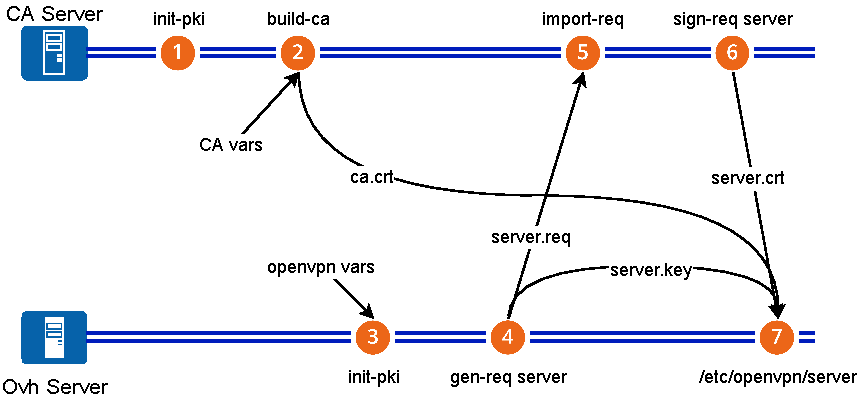
\includegraphics[width=1\linewidth]{immagini/diag-firma_certificato_ca}
    \caption{Diagramma per schematizzare la procedura di creazione della CA e della PKI del server OpenVPN.}
    \label{fig:diag-firma_certificato_ca}
\end{figure}


\subsection{Creazione della struttura di cartelle necessaria per ospitare la PKI \ok}
\label{subsec:pki_structure}

\begin{comment}
easy-rsa is a CLI utility to build and manage a PKI CA. In laymen's terms, this means to create a root certificate authority, and request and sign certificates, including intermediate CAs and certificate revocation lists (CRL).
\end{comment}

\todo[va bene wrapper??? :joy:]

Per la gestione della PKI verrà usato il tool \href{https://github.com/OpenVPN/easy-rsa}{\textit{easy-rsa}}, che fornisce un wrapper intorno alle funzionalità di \textit{OpenSSL} facilitandone l'utilizzo.

Il pacchetto \textit{easy-rsa} è presente nei repository ufficiali di ubuntu e può essere installato con il comando \code{sudo apt-get install easy-rsa}.


\begin{comment}
ln è un comando dei sistemi operativi Unix e Unix-like, e più in generale dei sistemi POSIX[1], che crea collegamenti simbolici e collegamenti fisici a file e directory. Se non diversamente specificato, crea collegamenti fisici. 
\end{comment}

Dopo l'installazione verrà creata una struttura di cartelle pronta a ospitare la PKI nel percorso \code{/usr/share/easy-rsa/}, ma è sconsigliato usarla per motivi di sicurezza. 

Quindi si deve spostare/collegare questo percorso in una cartella di un utente non privilegiato, andiamo quindi a crearne un collegamento nella home dell'utente \code{ubuntu}:

\begin{bashcode}{Server CA}{init-easyrsa}
$ mkdir ~/openvpn-ca
$ ln -s /usr/share/easy-rsa/* ~/openvpn-ca/ # soft link di easy-rsa nella home
$ chmod 700 /home/ubuntu/openvpn-ca/        # cambio i permessi in modo che solo l'utente
                                            #  corrente possa leggere il contenuto
\end{bashcode}

A questo punto possiamo usare lo script \code{easyrsa} presente nella cartella per creare la PKI.

\begin{bashcode}{Server CA}{}
$ tree ~/openvpn-ca/
.
|-- easyrsa -> /usr/share/easy-rsa/easyrsa
|-- openssl-easyrsa.cnf -> /usr/share/easy-rsa/openssl-easyrsa.cnf
|-- vars.example -> /usr/share/easy-rsa/vars.example
`-- x509-types -> /usr/share/easy-rsa/x509-types
\end{bashcode}



\begin{comment}

solo init-pki
\begin{bashcode}{Server CA}{}
tree
.
|-- easyrsa -> /usr/share/easy-rsa/easyrsa
|-- openssl-easyrsa.cnf -> /usr/share/easy-rsa/openssl-easyrsa.cnf
|-- vars.example -> /usr/share/easy-rsa/vars.example
`-- x509-types -> /usr/share/easy-rsa/x509-types

1 directory, 3 files
\end{bashcode}

build-ca
\begin{bashcode}{Server CA}{}
tree
.
|-- easyrsa -> /usr/share/easy-rsa/easyrsa
|-- openssl-easyrsa.cnf -> /usr/share/easy-rsa/openssl-easyrsa.cnf
|-- pki
|   |-- certs_by_serial
|   |-- index.txt
|   |-- index.txt.attr
|   |-- issued
|   |-- openssl-easyrsa.cnf
|   |-- private
|   |-- renewed
|   |   |-- certs_by_serial
|   |   |-- private_by_serial
|   |   `-- reqs_by_serial
|   |-- reqs
|   |-- revoked
|   |   |-- certs_by_serial
|   |   |-- private_by_serial
|   |   `-- reqs_by_serial
|   |-- safessl-easyrsa.cnf
|   `-- serial
|-- vars
|-- vars.example -> /usr/share/easy-rsa/vars.example
`-- x509-types -> /usr/share/easy-rsa/x509-types

14 directories, 9 files
\end{bashcode}

finale conf
\begin{bashcode}{Server CA}{}
$ tree
    .
    |-- easyrsa -> /usr/share/easy-rsa/easyrsa
    |-- openssl-easyrsa.cnf -> /usr/share/easy-rsa/openssl-easyrsa.cnf
    |-- pki
    |   |-- ca.crt
    |   |-- certs_by_serial
    |   |-- index.txt
    |   |-- index.txt.attr
    |   |-- issued
    |   |-- openssl-easyrsa.cnf
    |   |-- private
    |   |   `-- ca.key
    |   |-- renewed
    |   |   |-- certs_by_serial
    |   |   |-- private_by_serial
    |   |   `-- reqs_by_serial
    |   |-- reqs
    |   |-- revoked
    |   |   |-- certs_by_serial
    |   |   |-- private_by_serial
    |   |   `-- reqs_by_serial
    |   |-- safessl-easyrsa.cnf
    |   `-- serial
    |-- vars
    |-- vars.example -> /usr/share/easy-rsa/vars.example
    `-- x509-types -> /usr/share/easy-rsa/x509-types
    
    14 directories, 11 files
\end{bashcode}

finale totale
\begin{bashcode}{Server CA}{}
tree
.
|-- easyrsa -> /usr/share/easy-rsa/easyrsa
|-- openssl-easyrsa.cnf -> /usr/share/easy-rsa/openssl-easyrsa.cnf
|-- pki
|   |-- ca.crt
|   |-- certs_by_serial
|   |   |-- 7C4687A21AB7AF03EFD93FFC7D173C79.pem
|   |   |-- 8815692DCE6D78E99B25A6210DAEDBCB.pem
|   |   `-- FA98C8E3C0281617842ECEE92C2B13E7.pem
|   |-- index.txt
|   |-- index.txt.attr
|   |-- index.txt.attr.old
|   |-- index.txt.old
|   |-- issued
|   |   |-- client1.crt
|   |   |-- router1.crt
|   |   `-- server.crt
|   |-- openssl-easyrsa.cnf
|   |-- private
|   |   `-- ca.key
|   |-- renewed
|   |   |-- certs_by_serial
|   |   |-- private_by_serial
|   |   `-- reqs_by_serial
|   |-- reqs
|   |   |-- client1.req
|   |   |-- router1.req
|   |   `-- server.req
|   |-- revoked
|   |   |-- certs_by_serial
|   |   |-- private_by_serial
|   |   `-- reqs_by_serial
|   |-- safessl-easyrsa.cnf
|   |-- serial
|   `-- serial.old
|-- vars
|-- vars.example -> /usr/share/easy-rsa/vars.example
`-- x509-types -> /usr/share/easy-rsa/x509-types

14 directories, 23 files
\end{bashcode}
\end{comment}


\subsection{Creazione della \textit{Certificate Authority} CA \ok} % step 1, 2

Il primo step è la creazione della \textit{Certificate Authority}, passaggio 1 fig.\ref{fig:diag-firma_certificato_ca}. 

Andiamo quindi a usare l'albero di cartelle creato in code:~\ref{code:init-easyrsa}:

\begin{bashcode}{Server CA}{}
$ cd openvpn-ca/
$ ./easyrsa init-pki
init-pki complete; you may now create a CA or requests.
Your newly created PKI dir is: /home/ubuntu/openvpn-ca/pki
\end{bashcode}

Ora si devono personalizzare le variabili \code{vars}, si può sia partire da un file vuoto oppure modificare \code{vars.example} per poi rinominarlo \code{vars}.

Andiamo quindi a creare un nuovo file \code{vars}:

\todo[è ok lasciare queste?]

\begin{bashcode}{Server CA}{}
$ vim vars
set_var EASYRSA_REQ_COUNTRY  "IT"
set_var EASYRSA_REQ_PROVINCE "MC"
set_var EASYRSA_REQ_CITY     "Recanati"
set_var EASYRSA_REQ_ORG      "Esse-ti"
set_var EASYRSA_REQ_EMAIL    "s.gasparrini@esse-ti.it"
set_var EASYRSA_REQ_OU       "Esse-ti"
set_var EASYRSA_REQ_CN       "openvpn-ca"

set_var EASYRSA_ALGO         "ec"
set_var EASYRSA_DIGEST       "sha512"
\end{bashcode}

Le variabili nel primo blocco determinano i dati che poi verranno registrati nei certificati. Le ultime 2 sono opzioni di sicurezza. In particolare si setta il tipo di algoritmo di cifratura per usare la crittografia a chiave ellittica (\href{https://en.wikipedia.org/wiki/Elliptic-curve_cryptography}{Elliptic-Curve Cryptography}); L'ultima opzione setta l'algoritmo di hashing da usare nella firma dei certificati.

A questo punti si deve lanciare il comando \code{build-ca} per costruire la CA (passaggio 2 fig.\ref{fig:diag-firma_certificato_ca}):

\begin{bashcode}{Server CA}{}
$ ./easyrsa build-ca

Note: using Easy-RSA configuration from: ./vars

Using SSL: openssl OpenSSL 1.1.1f  31 Mar 2020

Enter New CA Key Passphrase: 
Re-Enter New CA Key Passphrase: 
read EC key
writing EC key

You are about to be asked to enter information that will be incorporated
into your certificate request.
What you are about to enter is what is called a Distinguished Name or a DN.
There are quite a few fields but you can leave some blank
For some fields there will be a default value,
If you enter '.', the field will be left blank.
-----
Common Name (eg: your user, host, or server name) [Easy-RSA CA]:

CA creation complete and you may now import and sign cert requests.
Your new CA certificate file for publishing is at:
/home/ubuntu/openvpn-ca/pki/ca.crt
\end{bashcode}

Eseguendo il comando verrà chiesto di inserire una passphrase, che verrà usata per cifrare la chiave privata appena generata. Se non si vuole cifrare la chiave privata, basta lasciare il campo vuoto. Il secondo prompt è relativo al \textit{Common Name} da dare alla certificazione, in questo caso è stato lasciato il valore di default \code{Easy-RSA CA}.

\subsection{Configurazione della PKI di OpenVPN \ok} % step 3, 4
\label{sec:pki_openvpn}

Il procedimento è simile al precedente, ma questa volta va eseguito sul \textit{Server}.

Quindi per prima cosa si devono ripetere i passaggi fatti in sezione \ref{subsec:pki_structure}, questa volta però chiamiamo la cartella \code{openvpn-pki} in modo da distinguerle:

\begin{bashcode}{Server}{}
$ mkdir openvpn-pki
$ ln -s /usr/share/easy-rsa/* ~/openvpn-pki/
$ chmod 700 /home/ubuntu/openvpn-pki/
$ cd openvpn-pki/
\end{bashcode}

Andiamo a creare un file \code{vars}, che questa volta contiene solo le informazioni essenziali, e poi dare il comando \code{init-pki} (step 3 fig.\ref{fig:diag-firma_certificato_ca}):

% step 3
\begin{bashcode}{Server}{}
$ vim vars
set_var EASYRSA_ALGO    "ec"
set_var EASYRSA_DIGEST  "sha512"
$ ./easyrsa init-pki
Note: using Easy-RSA configuration from: ./vars

init-pki complete; you may now create a CA or requests.
Your newly created PKI dir is: /home/ubuntu/openvpn-pki/pki
\end{bashcode}

A questo punto il server OpenVPN ha tutti i prerequisiti per creare una sua chiave privata e relativa \textit{Certificate Signing Request} (step 4 fig.\ref{fig:diag-firma_certificato_ca}). 

Come \textit{Common Name} è stato scelto \code{server}:

% step 4
\begin{bashcode}{Server}{}
$ ./easyrsa gen-req server nopass

Note: using Easy-RSA configuration from: ./vars

Using SSL: openssl OpenSSL 1.1.1f  31 Mar 2020
Generating an EC private key
writing new private key to '/home/ubuntu/openvpn-pki/pki/private/server.key.438W2xM0g9'
-----
You are about to be asked to enter information that will be incorporated
into your certificate request.
What you are about to enter is what is called a Distinguished Name or a DN.
There are quite a few fields but you can leave some blank
For some fields there will be a default value,
If you enter '.', the field will be left blank.
-----
Common Name (eg: your user, host, or server name) [server]:

Keypair and certificate request completed. Your files are:
req: /home/ubuntu/openvpn-pki/pki/reqs/server.req
key: /home/ubuntu/openvpn-pki/pki/private/server.key
\end{bashcode}

La chiave \code{server.key} va copiata nella cartella del server OpenVPN:

\begin{bashcode}{Server}{}
$ sudo cp /home/ubuntu/openvpn-pki/pki/private/server.key /etc/openvpn/server/
\end{bashcode}

Il secondo file creato, \code{server.req}, corrisponde a una \textit{Certificate Signing Request (CSR)} che va firmata e validata dalla CA. 

\subsection{Firma del certificato OpenVPN dalla CA \ok} % step 5, 6, 7
\label{subsec:sign_openvpn}

Per firmare la \textit{Certificate Signing Request} si deve copiare il file \code{.req} nel \textit{Server CA}, supponiamo quindi di averlo copiato nella cartella \code{/tmp}.

Ora lo si deve importare nella CA e firmarlo, ciò corrisponde ai passaggi 5 e 6 fig.\ref{fig:diag-firma_certificato_ca}:

% step 5, 6
\begin{bashcode}{Server CA}{}  
$ cd ~/openvpn-ca
$ ./easyrsa import-req /tmp/server.req server   # passaggio 5
$ ./easyrsa sign-req server server              # passaggio 6
Using configuration from /home/ubuntu/openvpn-ca/pki/safessl-easyrsa.cnf
Check that the request matches the signature
Signature ok
The Subject\'s Distinguished Name is as follows
commonName            :ASN.1 12:'server'
Certificate is to be certified until Mar 11 15:50:45 2025 GMT (1080 days)

Write out database with 1 new entries
Data Base Updated
\end{bashcode}

Verrà creato un file in \code{~/openvpn-ca/pki/issued} chiamato \code{server.crt}, che contiene il certificato firmato dalla CA.

Per concludere la procedura (step 7 fig.\ref{fig:diag-firma_certificato_ca}), si devono copiare i file \code{ca.crt} e \code{server.crt} dal \textit{Server CA} al \textit{Server OpnenVPN}, spostandoli nella cartella del \textit{Server OpenVPN}: \\\code{/etc/openvpn/server}.


\begin{comment}
finale

tree
.
|-- easyrsa -> /usr/share/easy-rsa/easyrsa
|-- openssl-easyrsa.cnf -> /usr/share/easy-rsa/openssl-easyrsa.cnf
|-- pki
|   |-- openssl-easyrsa.cnf
|   |-- private
|   |   |-- client1.key
|   |   `-- server.key
|   |-- reqs
|   |   |-- client1.req
|   |   `-- server.req
|   `-- safessl-easyrsa.cnf
|-- ta.key
|-- vars
|-- vars.example -> /usr/share/easy-rsa/vars.example
`-- x509-types -> /usr/share/easy-rsa/x509-types

4 directories, 13 files
\end{comment}

\section{Generazione della \textit{tls-crypt pre-shared key} \ok}
\label{sec:tls-crypt}

Per aumentare ulteriormente la sicurezza del nostro \textit{Server OpenVPN} possiamo creare un'ulteriore chiave, che permette di offuscare il certificato in fase di validazione. In questo caso la chiave è di tipo \textit{preshared} ed è comune per utti gli utenti, serve principalmente per aggiungere un ulteriore livello di sicurezza.

La creazione va fatta sul \textit{Server OpenVPN} e il file risultante va copiato nella cartella del server OpenVPN:

\begin{bashcode}{Server}{}
$ cd ~/openvpn-pki/
$ openvpn --genkey --secret ta.key
$ sudo cp ta.key /etc/openvpn/server
\end{bashcode}

\section{Generazione dei certificati per i \textit{clients} \ok}
\label{sec:client_keys}

La generazione dei certificati per i client consiste in una procedura molto simile alla creazione del certificato del \textit{Server}, sezione \ref{sec:pki_openvpn} e \ref{subsec:sign_openvpn}.

\begin{figure}[H]
    \centering
    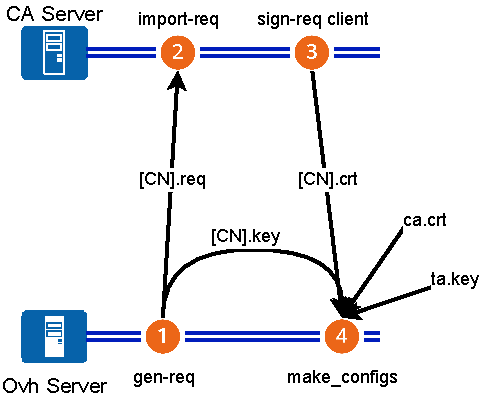
\includegraphics[width=0.6\linewidth]{immagini/diag-firma_certificato_client}
    \caption{Diagramma per schematizzare la procedura di firma di un certificato client.}
    \label{fig:diag-firma_certificato_client}
\end{figure}

Per ospitare i certificati dei client e le loro chiavi, creiamo una cartella nella home. Successivamente verrà usata per automatizzare la creazione dei file di configurazione OpenVPN che verranno usati dai client per connettersi alla VPN.

\begin{bashcode}{Server}{clients-config-folder}
$ mkdir -p ~/client-configs/keys
$ chmod -R 700 ~/client-configs
\end{bashcode}

Creiamo quindi un certificato per un \textit{Client}, è importante che il \textit{Common Name} dato al certificato sia unico ed è consigliabile usare un nome che permetta di collegare il certificato con il cliente che ha richiesto il servizio. Ciò permette di conoscere quale certificato revocare in caso sia necessario \cite{revoke-cert}.

In questo caso è stato usato il \textit{Common Name} \code{client1} (step 1 fig.\ref{fig:diag-firma_certificato_client}):

\begin{bashcode}{Server}{}
$ cd ~/openvpn-pki/
$ ./easyrsa gen-req client1 nopass
\end{bashcode}

Con questo comando verranno creati 2 file: 
\begin{itemize}
    \item \code{pki/private/client1.key} costituisce la chiave privata del certificato e va copiata nella cartella creata in code:~\ref{code:clients-config-folder};
    \item \code{pki/reqs/client1.req} è la \textit{Certificate Signing Request} che deve essere copiata nel \mbox{\textit{Server CA}} per essere firmata.
\end{itemize}

Supponiamo di aver copiato il file \code{client1.req} nella cartella \code{tmp} del \textit{Server CA}, possiamo quindi importarla e firmarla (passaggi 2 e 3 fig.\ref{fig:diag-firma_certificato_client}):

\begin{bashcode}{Server CA}{}
$ cd ~/openvpn-ca
$ ./easyrsa import-req /tmp/client1.req client1     # passaggio 2
$ ./easyrsa sign-req client client1                 # passaggio 3
Using configuration from /home/ubuntu/openvpn-ca/pki/safessl-easyrsa.cnf
Check that the request matches the signature
Signature ok
The Subject\'s Distinguished Name is as follows
commonName            :ASN.1 12:'client1'
Certificate is to be certified until Mar 16 13:15:09 2025 GMT (1080 days)

Write out database with 1 new entries
Data Base Updated
\end{bashcode}

Ciò produrrà il file di certificato \code{openvpn-ca/pki/issued/client1.crt} che deve essere copiato nel \textit{Server OpenVpn}, supponiamo di copiarlo nella cartella \code{~/client-configs/keys/}.

\subsection{Script per la creazione delle configurazioni dei client \ok}
\label{subsec:script_client}

Per facilitare la creazione dei file di configurazione dei client, \code{Common-Name.ovpn}, andremo a creare un apposito script bash che userà la cartella creata in code:\ref{code:clients-config-folder}. 

Per concludere la preparazione si devono copiare i file \code{ta.key} (creato nella sezione \ref{sec:tls-crypt}) e \code{ca.crt} (creato nella sezione \ref{subsec:sign_openvpn}), sistemando inoltre l'\textit{owner} in modo che l'utente non privilegiato vi possa accedere:

\begin{bashcode}{Server}{}
$ cp ~/openvpn-pki/ta.key ~/client-configs/keys/
$ sudo cp /etc/openvpn/server/ca.crt ~/client-configs/keys/
$ sudo chown ubuntu:ubuntu ~/client-configs/keys/*
\end{bashcode}

Ora andiamo a scaricare e personalizzare la configurazione di esempio per i client:

\begin{bashcode}{Server}{}
$ cd ~/client-configs/
$ wget "https://raw.githubusercontent.com/OpenVPN/openvpn\
            /master/sample/sample-config-files/client.conf" \
                -O base.conf
$ vim base.conf
42   remote 51.178.141.119 1194     # va messo l'IP e la porta del server OpenVPN
88   ;ca ca.crt                     # non useremo i file esterni ma ingloberemo 
89   ;cert client.crt               #   questi file direttamente nella
90   ;key client.key                #   configurazione del client
108  ;tls-auth ta.key 1             # 
116  cipher AES-256-GCM             # cifratura usata
117  auth SHA256                    # autenticazione usata
118  key-direction 1                # indica che è un client
\end{bashcode}

Ora creiamo lo script bash \code{make_config.sh}:

\begin{bashcode}{Server}{}
$ vim make_config.sh
#!/bin/bash

# usage:
# \$ make\_config.sh client1
# will use [ca.crt, client1.crt, client1.key, ta.key] to create client1.ovpn
    
KEY_DIR=~/client-configs/keys
OUTPUT_DIR=~/client-configs/files
BASE_CONFIG=~/client-configs/base.conf
    
cat ${BASE_CONFIG} \
    <(echo -e '<ca>') \
    ${KEY_DIR}/ca.crt \
    <(echo -e '</ca>\n<cert>') \
    ${KEY_DIR}/${1}.crt \
    <(echo -e '</cert>\n<key>') \
    ${KEY_DIR}/${1}.key \
    <(echo -e '</key>\n<tls-crypt>') \
    ${KEY_DIR}/ta.key \
    <(echo -e '</tls-crypt>') \
    > ${OUTPUT_DIR}/${1}.ovpn
$ chmod 700 make_config.sh
\end{bashcode}

Questo script permette di aggiungere in modo \textit{inline} i file necessari all'autenticazione di un client alla VPN, ha il vantaggio di poter inviare al cliente un solo file invece di 5.

Quindi, in base al \textit{Common Name} passato come argomento, lo script userà: il certificato della CA, \code{ca.crt}; 
il certificato e chiave relativi al \textit{Client} per cui si sta creando la configurazione, usando il \textit{Common Name} passato come argomento; 
e la \textit{preshared key}, \code{ta.key}.

Il tutto viene scritto in un file che ha lo stesso nome del \textit{Common Name} del \textit{Client} per cui si sta creando la configurazione ma con estensione \code{.ovpn}.

Quindi per creare la configurazione di \textit{client1} (passaggio 4 fig.\ref{fig:diag-firma_certificato_client}):

\begin{bashcode}{Server}{config-client1}
$ ./make_config.sh client1
\end{bashcode}

Ciò creerà il file \code{client-configs/files/client1.ovpn}, successivamente sarà necessario copiare questo file nella macchina del \textit{Client}.

\section{Creazione del file di configurazione del Server OpenVPN \ok}
\label{sec:server_config}

Il server openvpn viene configurato attraverso il file di configurazione \\\code{/etc/openvpn/server/server.conf}, per non partire da una configurazione vuota si può usare la configurazione di esempio offerta da OpenVPN:

\begin{bashcode}{Server}{}
$ cd /etc/openvpn/server/
$ sudo wget "https://raw.githubusercontent.com/OpenVPN/openvpn/\
                master/sample/sample-config-files/server.conf"
\end{bashcode}

A questo punto andiamo a modificare il file di esempio personalizzandolo per le nostre necessità, per facilitare la riproduzione di questa configurazione è stato aggiunto il numero della riga che è stata modificata:

\begin{bashcode}{Server}{}
$ sudo vim server.conf
85  dh none             # non sono stati usati i parametri Diffie-Hellman
92  topology subnet     # topologia raccomandata
244 ;tls-auth ta.key 0  # questa riga va commentata
245 tls-crypt ta.key    # selezione della preshared key
253 cipher AES-256-GCM  # selezione della cifratura scelta
275 user nobody         # utente che eseguirà il server openvpn, in modo da 
                        #  restringere i permessi
276 group nogroup       # stassa cosa per il gruppo
318 auth sha256         # selezione del metodo di autenticazione
\end{bashcode}


\section{Configurazioni sulla network stack del Server \ok}
\label{sec:network_stack}

OpenVPN per funzionare necessita che il server abbia l'\textit{ip forwarding} abilitato. Ciò è necessario per permettere al server OpnenVPN di inoltrare il traffico proveniente dalla VPN nella sua network stack, e viceversa.

\begin{comment}
Now your OpenVPN server will be able to forward incoming traffic from one ethernet device to another. This setting makes sure the server can direct traffic from clients that connect on the virtual VPN interface out over its other physical ethernet devices. This configuration will route all web traffic from your client via your server’s IP address, and your client’s public IP address will effectively be hidden.
\end{comment}


Per abilitare l'\textit{ip forwarding} nella network stack si dovrà modificare il file \code{/etc/sysctl.conf}, il successivo comando serve a ricaricare le configurazioni dai file:

\begin{bashcode}{Server}{}
$ sudo vim /etc/sysctl.conf
69 net.ipv4.ip_forward = 1
$ sudo sysctl -p
net.ipv4.ip_forward = 1
\end{bashcode}

\section{Configurazione del firewall \ok}
\label{sec:firewall}

Sulla VPS scelta (sezione \ref{subsec:vps-ovhcloud}) è presente il firewall \code{firewalld}, ma per una più semplice configurazione è consigliato di disattivarlo e installare \code{ufw}:

\begin{bashcode}{Server}{}
$ sudo systemctl mask firewalld
$ sudo systemctl stop firewalld
$ sudo apt-get install ufw
$ sudo ufw allow ssh
Rule added
Rule added (v6)
$ sudo ufw enable
\end{bashcode}

È importantissimo abilitare l'SSH prima di abilitare il firewall, altrimenti si perderà l'accesso alla VPS.

\subsection{Configurazione del NAT \ok}

Per far si che i pacchetti provenienti dalla VPN entrino nella network stack del \textit{Server} si deve aggiungere una regola di NAT nel firewall. Per farlo si deve conoscere quale è l'interfaccia di rete del \textit{Server}, cioè quella che ha come IP il suo IP pubblico:

\begin{bashcode}{Server}{}
$ ip addr
[...]
2: ens3: <BROADCAST,MULTICAST,UP,LOWER_UP> mtu 1500 qdisc mq state UP group default qlen 1000
    link/ether a6:23:5f:48:ba:de brd ff:ff:ff:ff:ff:ff
    inet 51.178.141.119/20 brd 51.178.141.255 scope global dynamic ens3
       valid_lft 1857sec preferred_lft 1857sec
    inet6 fe80::23:bfff:ac24:aace/64 scope link
       valid_lft forever preferred_lft forever
[...]
\end{bashcode}

In questo caso il nome dell'interfaccia di rete è \textit{ens3}. Possiamo quindi procedere con la configurazione del NAT:

\begin{bashcode}{Server}{}
$ sudo vim /etc/ufw/before.rules
# ## rules.before
# ## Rules that should be run before the ufw command line added rules. Custom
# rules should be added to one of these chains:
# ufw-before-input
# ufw-before-output
# ufw-before-forward
#

# START OPENVPN RULES
# NAT table rules
*nat
:POSTROUTING ACCEPT [0:0]
# Allow traffic from OpenVPN client to ens3 
-A POSTROUTING -s 10.8.0.0/24 -o ens3 -j MASQUERADE
COMMIT
# END OPENVPN RULES


# Don't delete these required lines, otherwise there will be errors
*filter
. . .
\end{bashcode}

Nella modifica del file si deve stare attenti a inserire la nuova regola in cima al file e sotto i commenti iniziali, è inoltre importante inserire i commenti nella regola.

\subsection{Configurazione del packet forwarding \ok}

Precedentemente abbiamo abilitato il forwarding nella network stack del server (sezione \ref{sec:network_stack}), ora si deve abilitare la corrispondente opzione nel firewall. Si deve quindi cambiare la regola di default per i pacchetti inoltrati da \code{DROP} ad \code{ACCEPT}.

Per farlo si deve modificare il file \code{/etc/default/ufw}:

\begin{bashcode}{Server}{}
$ sudo vim /etc/default/ufw
DEFAULT_FORWARD_POLICY="ACCEPT"
\end{bashcode}


\subsection{Conclusione della configurazione del firewall \ok}

Per concludere la configurazione si deve abilitare la porta relativa alla vpn, in questo caso \code{1194}, e riavviare il firewall:

\begin{bashcode}{Server}{}
$ sudo ufw allow 1194/udp
$ sudo ufw reload
$ sudo ufw status
Status: active
To              Action      From
--              ------      ----
22              ALLOW       Anywhere
1194/udp        ALLOW       Anywhere
22 (v6)         ALLOW       Anywhere (v6)
1194/udp (v6)   ALLOW       Anywhere (v6)
\end{bashcode}

Se la configurazione è stata effettuata correttamente di avrà un output simile al precedente, in caso contrario si dovranno valutare gli errori dati da ufw.

\section{Avvio del Server OpenVPN \ok}
\label{sec:start_server}

Ora che la configurazione del Server è in una situazione stabile possiamo tentate di avviarlo:

\begin{bashcode}{Server}{}
$ sudo systemctl enable openvpn-server@server.service
$ sudo systemctl start openvpn-server@server.service
$ sudo systemctl status openvpn-server@server.service
● openvpn-server@server.service - OpenVPN service for server
     Loaded: loaded (/usr/lib/systemd/system/openvpn-server@.service; enabled; vendor preset: disabled)
     Active: active (running) since Mon 2022-04-18 13:08:44 CEST; 4h 22min ago
       Docs: man:openvpn(8)
             https://community.openvpn.net/openvpn/wiki/Openvpn24ManPage
             https://community.openvpn.net/openvpn/wiki/HOWTO
   Main PID: 436 (openvpn)
     Status: "Initialization Sequence Completed"
      Tasks: 1 (limit: 9488)
     Memory: 4.8M
        CPU: 199ms
     CGroup: /system.slice/system-openvpn\x2dserver.slice/openvpn-server@server.service
             └─436 /usr/bin/openvpn --status /run/openvpn-server/status-server.log --status-version 2 --suppress-timestamps --config server.conf

Apr 18 13:08:44 server openvpn[436]: TUN/TAP device tun0 opened
Apr 18 13:08:44 server openvpn[436]: Incoming Control Channel Encryption: Cipher 'AES-256-CTR' initialized with 256 bit key
Apr 18 13:08:44 server openvpn[436]: Incoming Control Channel Encryption: Using 256 bit message hash 'SHA256' for HMAC authentication
Apr 18 13:08:44 server openvpn[436]: net_addr_v4_add: 10.8.0.1/24 dev tun0
Apr 18 13:08:44 server openvpn[436]: UDPv4 link local (bound): [AF_INET][undef]:1194
Apr 18 13:08:44 server openvpn[436]: UDPv4 link remote: [AF_UNSPEC]
Apr 18 13:08:44 server openvpn[436]: MULTI: multi_init called, r=256 v=256
Apr 18 13:08:44 server openvpn[436]: IFCONFIG POOL IPv4: base=10.8.0.2 size=253
Apr 18 13:08:44 server openvpn[436]: IFCONFIG POOL LIST
Apr 18 13:08:44 server openvpn[436]: Initialization Sequence Completed
\end{bashcode}
 
Il comando \code{systemctl enable} abilita il servizio per essere avviato all'avvio della macchina, mentre \code{systemctl start} lo avvia immediatamente. 

Con il comando \code{systemctl status} si può verificare lo stato del servizio, si vede che il servizio è \textit{active (running)}. 

In caso il servizio fallisse ad avviarsi si avrà un breve log con \code{systemctl status}, oppure si possono leggere i log completi usando \code{journalctl -u openvpn-server@server.service}.


\section{Test della configurazione \ok}
\label{sec:test_config_server}

Ora che la configurazione per questo capitolo è conclusa possiamo testare che tutto funzioni correttamente.

Per farlo ci spostiamo su una macchina \textit{Client}, con sistema operativo Linux ad esempio. Usando la configurazione creata in code:\ref{code:config-client1} possiamo connettere il \textit{Client} alla VPN:

\begin{bashcode}{Client}{}
$ sudo openvpn --config client1.ovpn
[...]
Thu Apr 21 12:53:04 2022 Outgoing Data Channel: Cipher 'AES-256-GCM' initialized with 256 bit key
Thu Apr 21 12:53:04 2022 Incoming Data Channel: Cipher 'AES-256-GCM' initialized with 256 bit key
Thu Apr 21 12:53:04 2022 ROUTE_GATEWAY 192.168.1.20/255.255.255.0 IFACE=eth0 HWADDR=02:42:0a:00:04:03
Thu Apr 21 12:53:04 2022 /sbin/ip route add 10.8.0.1/32 via 10.8.0.2
Thu Apr 21 12:53:04 2022 WARNING: this configuration may cache passwords in memory -- use the auth-nocache option to prevent this
Thu Apr 21 12:53:04 2022 Initialization Sequence Completed
\end{bashcode}

Se la configurazione fino a questo punto è corretta si avrà il messaggio \\\code{Initialization Sequence Completed}.

Nel \textit{Client} si avrà una nuova interfaccia di rete chiamata \code{tun0}, questa è l'interfaccia virtuale creata dalla vpn:

\begin{bashcode}{Client}{}
$ ip addr
2: tun0: <MULTICAST,NOARP,UP,LOWER_UP> mtu 1500 qdisc fq_codel state UNKNOWN group default qlen 500
    link/none 
    inet 10.8.0.2/24 scope global tun0
       valid_lft forever preferred_lft forever
\end{bashcode}

Si può vedere come l'IP assegnato al \textit{Client} dalla VPN è \code{10.8.0.2}.

Per testare che la connessione sia instaurata correttamente si può usare la utility \code{ping}, ad esempio possiamo fare il ping dal \textit{Client} verso l'IP interno alla VPN del \textit{Server}:

\begin{bashcode}{Client}{}
$ ping -c1 10.8.0.1
PING 10.8.0.1 (10.8.0.1) 56(84) bytes of data.
64 bytes from 10.8.0.1: icmp_seq=1 ttl=64 time=0.250 ms
\end{bashcode}

Se nel frattempo si esegue la utility \code{tpcdump} sul server si potranno vedere i pacchetti \textit{echo request} ed \textit{echo reply}:

\begin{bashcode}{Server}{}
$ sudo tcpdump -i tun0
listening on tun0, link-type RAW (Raw IP), capture size 262144 bytes
13:11:12.018615 IP 10.8.0.2 > 10.8.0.1: ICMP echo request, id 11, seq 1, length 64
13:11:12.018640 IP 10.8.0.1 > 10.8.0.2: ICMP echo reply, id 11, seq 1, length 64
\end{bashcode}

Si vede quindi che è possibile instaurare una comunicazione bidirezionale tra \textit{Client}, \code{10.8.0.2}, e \textit{Server}, \code{10.8.0.1}.

Abbiamo quindi realizzato correttamente la topologia di obbiettivo per questo capitolo, descritta in fig.\ref{fig:diag-simple_ips_vpn}.


